\documentclass{article}

\usepackage{graphicx}
\usepackage{subcaption}
\usepackage[font=small,labelfont=bf]{caption}
\usepackage{array}
\newcolumntype{C}[1]{>{\centering\let\newline\\\arraybackslash\hspace{0pt}}m{#1}}
\begin{document}
	
	\title{Report of \textit{Jumeau numérique} project}
	\author{Rita Maestri, Solal Canqueteau}
	\maketitle
	
\newpage

\tableofcontents
\newpage

	
\part{Introduction}

The airport capacity, i.e. the number of aircraft that can depart or land on the airport surface by unit of time, is influenced by many factors, such as the airport infrastructures (number of runways and stands) and the heterogeneity of aircraft types on the airport platform (due to security distance issues) \cite{gotteland}.

The project \textit{jumeau numérique} has as an objective increasing the airport capacity by optimizing the efficiency of the taxiway, runway and stand usage procedures at Charles de Gaulle airport (CDG). In particular, the goal of the project is minimizing the taxi time, i.e. the time it takes for an aircraft to go from the stand to the runway or vice versa.

In literature, this task is accomplished with the help of simulations in two main ways \cite{rathinam}:

\begin{itemize}
	\item Holding aircraft at their gates as
	long as possible and then release them at the optimal TOBT (target off-block time, i.e. the time at witch an aircraft is supposed to begin the push back procedure)
	schedule. This method allows to limit the length of the queue at the runway and also to turn on the engine of the aircraft as late as possible, saving fuel and avoiding CO2 emissions.

	\item determine de-conflicted taxi routes to avoid the stop of an aircraft to give way to another one.
\end{itemize}

Both those methods require the implementation of an automatic support tool for air traffic control operators (ATCO), that suggest them an optimized schedule or an optimized taxi route. Furthermore, classical simulation methods are used to obtain the result.


On the contrary, the main purpose of our project is to investigate the human influence on taxi time.
In fact, the management of the traffic on runways, taxiways and parking stands is the main task of the ground controllers (GC). Consequently, the efficiency of the schedule and of the taxi routes depends heavily on their decisions.

Our work involve two parts, one as a function of the other. The data analysis is focused on the identification of patterns in the behavior of aircraft that use the airport platform and consequently in the strategy of GC. Once the strategies are well defined, with the help of interviews to GC and pilots, an ABM will be implemented. 

An ABM allows to integrate infrastructural and human/organizational factors in the same simulation. In fact, the airport platform can be modeled as the environment in which the GC, the aircraft and the other agents act and interact, following precise strategies.

\part{Airport traffic management}

\section{Turnaround operations}
All the operations that take place from the moment when an aircraft lands to the moment when it takes off are named turnaround operations. It is fundamental to know them to be able to analyze the airport traffic flow. 

An effective description of the turnaround operations is given in \cite{noortman}:

``Arriving aircraft receive a landing approval when they are on final approach. Once touched down, these aircraft should leave the runway as quickly as possible to make room for the next aircraft. A taxi route is allocated by ATC [air traffic control, author's note], which guides the aircraft towards its stand. In case the gate is not available (shortly), the aircraft is guided to a holding position such that it does not block taxiways for other aircraft. In air transportation the standard holds that aircraft coming from the right have priority.

Once an aircraft has arrived at its stand, ground handlers have to perform multiple actions to get the aircraft ready for its next flight. These operations include disembarking, refuelling, cleaning, catering and boarding. Although an aircraft has a scheduled time to be released from its stand, delays are likely because of e.g. the aircraft arriving late, limited availability of resources, severe weather conditions or restrictions from EUROCONTROL [an international organisation whose aim is to guarantee safe air traffic management across Europe, that coordinates the A-CDM project, described below, author's note].

Once ready, the departing aircraft notifies ATC and, if the situation allows, a start-up approval is given, followed by a push back approval. This allowance depends on multiple conditions, including whether vehicles and personnel have left the stand and whether direct push-back would be possible.
After its push back, the aircraft receives a taxi route and approval to taxi. Depending on its route, approval might be required to cross specific points in the airport infrastructure, including a runway. When arriving at the runway, the departing aircraft once again waits for approval from ATC to line up and take off."


At CDG airport, those operations involve many different agents and are coordinated thanks to the Airport-Collaborative Decision Making procedure (A-CDM).

\section{A-CDM and airport agents}\label{ACDM}
The A-CDM is an EUROCONTROL project that aims to ameliorate the information sharing between airport partners and consequently the efficiency of the airport. In particular, arrival predictability, TOBT predictability and Take-Off predictability are increased by the use of A-CDM procedure\cite{ACDMimpact}.

The main stakeholders involved in the A-CDM procedure are:
\begin{itemize}
	\item \textbf{Aircraft Operators} (Air France, Easy Jet...). They provide for flight plan data, TOBT, movement messages, etc.
	\item \textbf{Network Manager Operations Centre (NMOC)}: It provides for updates in flight plan, CTOT (Calculated Take-Off Time, based on the time slot in which a flight is allowed to take off), etc.
	\item \textbf{Air Traffic Controllers}. They provide for runway capacity, update in TOBT, etc.
	\item\textbf{Airport Operators.} They provide for estimated de-icing time, etc.
\end{itemize}

The operational core of A-CDM system is the pre-departure sequencer, also called Departure Manger (DMAN). The DMAN is a planning tool calculates the Target Take Off Times (TTOT) and the Target Startup Approval Times (TSAT, the time when an aircraft should begin the push-back procedure calculated by the DMAN) based on the information gained thanks to the A-CDM procedure.

\subsection{DMAN inputs}
The main goal of the DMAN is to calculate TSAT (Target Startup Approval Time) based on the TOBT (Target off block time, the time when an aircraft should begin the push-back procedure calculated by the Aircraft Operators), and TTOT, adding to the TSAT the estimated taxi time. 
When elaborating the pre-departure sequence the Basic DMAN takes into account \cite{DMAN}:
\begin{itemize}
\item Existing CFMU (Central Flow Management Unit, an EUROCONTROL organ) slots (CTOT, calculated off-block time): many aircraft must depart within a time interval of 15 minutes not to loose the clearance;
\item Variable Taxi Times (including remote de-icing times when needed), taken from a table of taxi times at CDG;
\item Basic runway constraints such as capacity and pressure, provided from the Tower Supervisor;
\item Aircraft Wake Vortex separations (optional);
\item Standard Instrument Departure (SID) and Minimum Departure Interval (MDI).
\end{itemize}

\subsection{DMAN output}

DMAN has an human-machine interface for Delivery Controllers, who are in charge of  of giving the departure clearance to the aircraft. The output of the DMAN consists in a list of flights that should begin their push-back in the next 45 minutes, with the respective suggested TSAT. The list is updated every 30 seconds.

The DMAN gives as an output also the suggested runway, that in exceptional cases can be changed by delivery or ground controller 15 minutes before the TSAT. In this case, the new runway is given as an input to the DMAN, that recomputes the departure sequence. 


\section{Actors}
Below is a table that lists the actors involved in the airport platform management and their responsibilities \cite{DMAN}.


\begin{figure}[h!!!!!!!!!!!!!!!!]

	\centering
	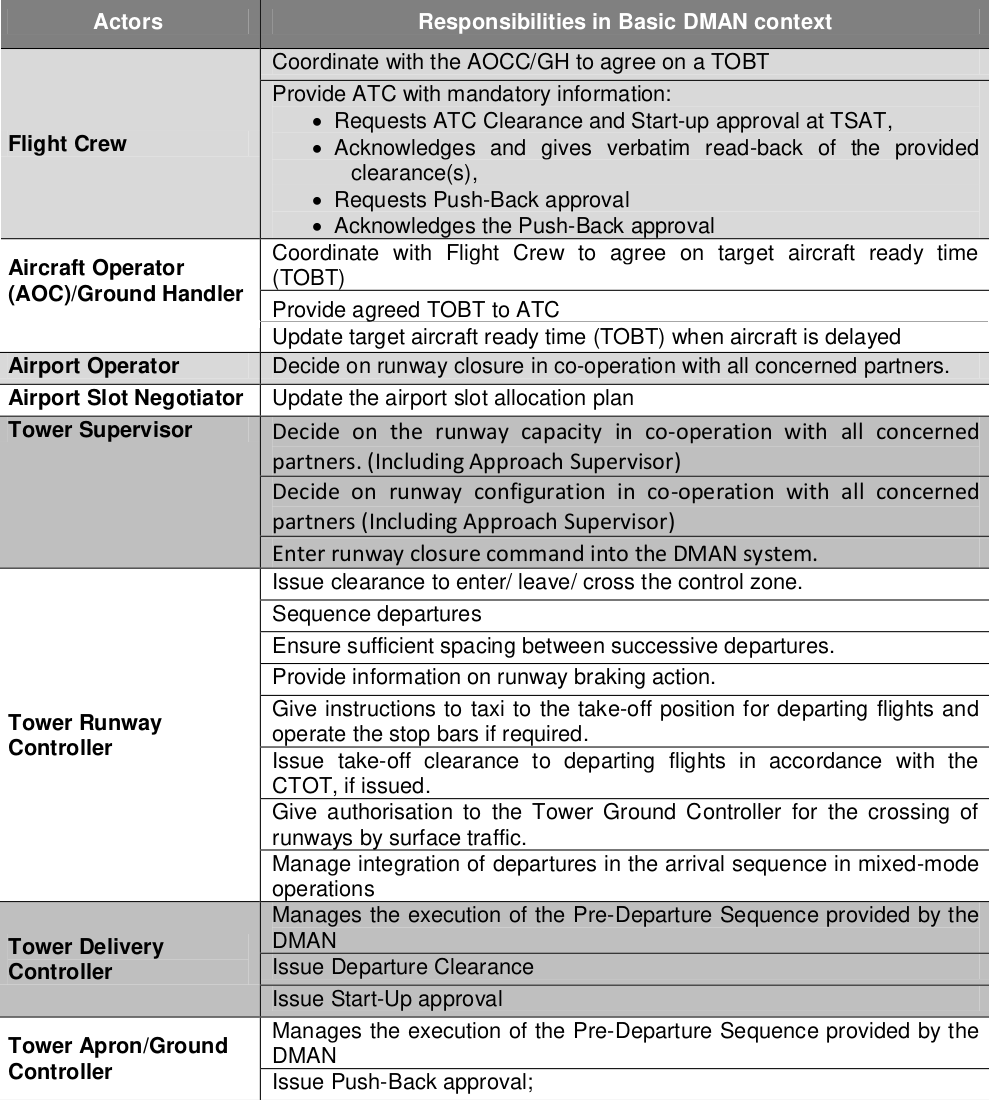
\includegraphics[width=9cm]{tabella.png}
	\caption{List of actors involved in turn around operations and their responsibility with respect to the DMAN system.}
	\label{actors}

\end{figure}

\bigskip
The table shows that there are 8 actors involved in the ground operations. One of the challenges of the ABM will be to simplify the complexity of interactions deriving from this organizational setting without losing accuracy.

\newpage
\part{Data Analysis}

The data analysis were performed on a data set provided by DGAC that contains information about 1059702 flights, that correspond to all the flights managed by CDG airport from 01/01/2018 to 29/02/2020.


\section{Exploratory analysis: Taxi time dependency on companies and associated stand}\label{exploratory}

One of the factors that could influence the pilots behavior, and consequently the taxi time, is the aircraft operator (air company). In fact, for example, we expect Air France pilots to be quicker in taxiing because they know the airport better. Another behavior that has been reported by CDG ATCOs is that Ryanair flights tended to declare to have run out of fuel to gain the priority in landing, even if it wasn't true. We tried to detect eventual inconsistencies in the taxi time for the most frequent users of CDG.

\subsection{Taxi time distribution for different companies}
Below is a plot of the histograms of taxi times for the 5 most frequent aircraft operators at CDG.

\bigskip
\begin{minipage}{\textwidth}
	\begin{minipage}[b]{0.5\textwidth}
		\centering
		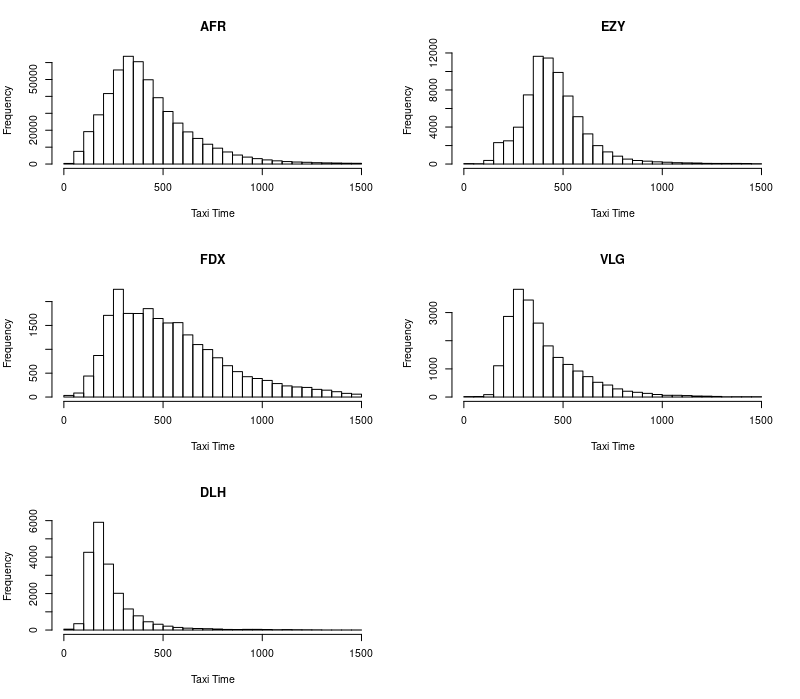
\includegraphics[scale=0.3]{companiesTaxiTime.png}
		\captionof{figure}{Histograms of taxi times for different companies at CDG.}
		\label{companiesFig}
	\end{minipage}
\hfill
	\begin{minipage}[b]{0.4\linewidth}
		\centering
		\tiny
		\begin{tabular}{p{0.8cm}p{1.3cm}p{0.8cm}p{0.6cm}}\hline
			Company & N° of flights over the total n° of flights & Mean Taxi Time(s) & $\sigma$ (s)\\ \hline
			AFR & 48\%& 433 s & 261 s\\
			EZY & 7\% & 460 s & 194 s\\
			FDX & 2\% & 548 s & 315 s\\ 
			VLG & 2\% & 403 s & 212 s\\
			DLH & 2\% & 240 s & 191 s\\
			\hline
		\end{tabular}
	\bigskip
	\bigskip
		\captionof{table}{Percentage over the total number of flights, avarage taxi time and relative standard deviation for the company whose flight are the most frequent at CDG.}
		\label{companiesTable}
	\end{minipage}
\end{minipage}
\bigskip

Figure \ref{companiesFig} and table \ref{companiesTable} show that different taxi times correspond to different companies.  

\subsection{Taxi time model}

Large taxi times can be caused by many events, like bad weather conditions, operational inefficiencies, aircraft malfunctioning, etc.. But in our approach to the data analysis, we decided to begin with a very simple model of taxi time, to identify which of the independent variables that the taxi time depends on is the major contributor.

The taxi time ($t_t$) can be modeled as ($t_t$):
\begin{equation}\label{time-eq}
t_t = \frac{d}{v} + t_{w}, 
\end{equation}
where $d$ is the distance traveled by the aircraft, $v$ is the aircraft speed, $t_{w}$ is the waiting time during taxiing.

As a first try, we tried to link the longer mean taxi time of some companies with the distance $d$.

\subsection{Taxi time VS taxi distance}\label{regression}
We performed a linear regression to verify the relation between the mean taxi time calculated over all the flights of a specific company and the respective mean taxi distance, that are shown in table \ref{tableDistances} for the most frequent user of CDG.

\begin{table}[h!!!!!!!!!!!!!!!!!!!!!!]
\centering

\begin{tabular}{p{1.5cm}p{1.5cm}p{1.6cm}}\hline
	Company & Mean Distance & Mean Taxi Time\\ \hline
	AFR & 3.22 NM & 433 s \\
	EZY & 3.30 NM & 460 s\\
	FDX & 3.78 NM & 548 s\\ 
	VLG & 3.03 NM & 403 s\\
	DLH & 2.32 NM & 240 s\\
	\hline
\end{tabular}
\captionof{table}{Mean taxi distance and mean taxi time for different companies.}
\label{tableDistances}
\end{table}

The linear regression gave the following result.

\begin{table}[h!!!!!!!!!!]
	\centering
	\begin{tabular}{p{1.5cm}p{1.5cm}p{1.5cm}p{1.4cm}p{1.7cm}}\hline
		 & Estimate & Standard Error& t value & p value ($Pr(>|t|)$) \\ \hline
		\smallskip Intercept & \smallskip -282.87 & \smallskip 34.93 & \smallskip -8.099s & \smallskip 9.18e-15\\
		 \smallskip Slope &\smallskip 244.32 &\smallskip 34.93 &\smallskip 21.526 &\smallskip < 2e-16\\

		\hline
	\end{tabular}

	\captionof{table}{Results of the linear regression.}
	\label{linearRegression}
\end{table}

Since the t value showed a statistically significant difference of our data with the null hypothesis, we can conclude that the differences in taxi times for the various companies are mostly due to the different distances traveled by the aircraft of these companies. 
In fact, at CDG a precise parking area in assigned, and some of them are more unfavorable than others in terms of taxi distance, as shown in section \ref{comparison}.


\subsection{Night time peak in taxi times}

If we plot the taxi time averaged over all the flights as a function of the hour of the day, we see a peak that cannot be explained by the number of aircraft that are crossing the taxiway (Figure ~\ref{n_avions}).

\begin{figure}[h]
	\centering
	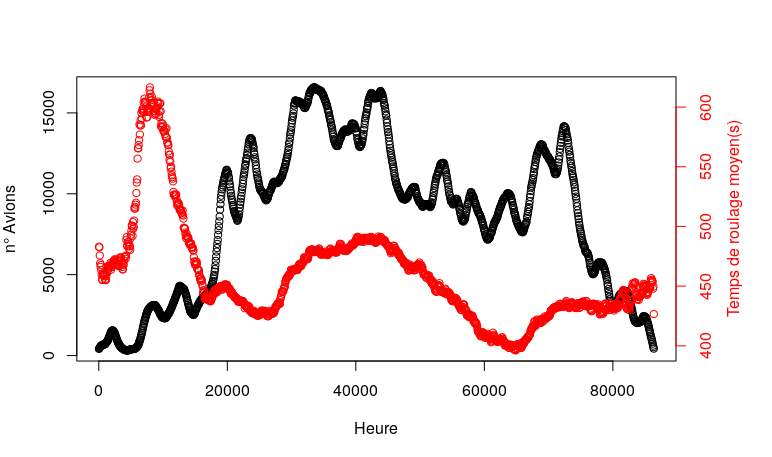
\includegraphics[width=8cm]{n_avions_TempsRoulage}
	\caption{Comparison between number of aircrafts in the taxiway (black line) and taxi time (red line).}
	\label{n_avions}
\end{figure}

So we performed an analysis of all the variables, included in equation \ref{time-eq}, that can contribute to the unexplained peak of 3 a.m

\begin{figure}[h!!!!!!!!!]
	\centering
	\begin{subfigure}[b]{0.5\textwidth}
		\centering
		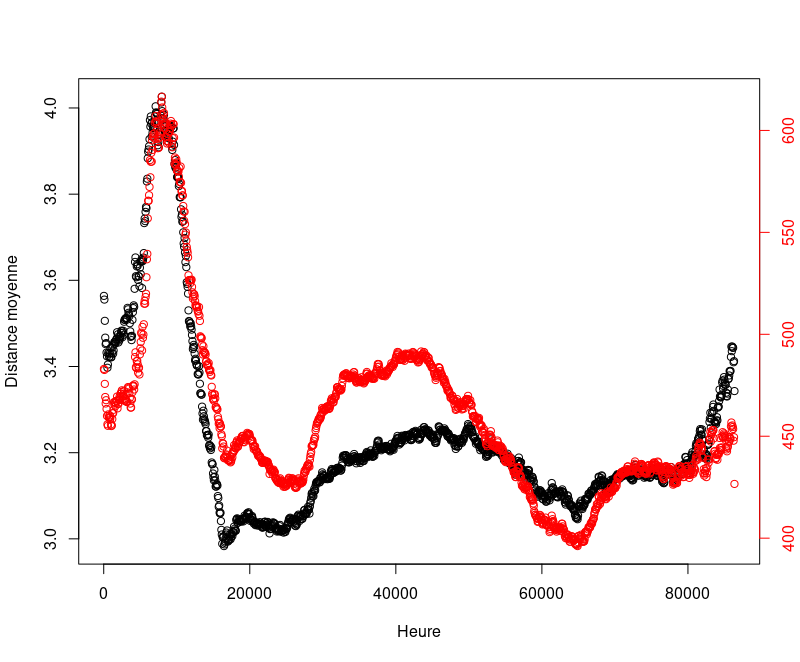
\includegraphics[width=5cm]{Distance}
		\caption{Comparison between distance of the parking from the runway (black) and taxi time (red).}
		\label{distance}
	\end{subfigure}
	\hfil
	\begin{subfigure}[b]{0.4\textwidth}
		\centering
		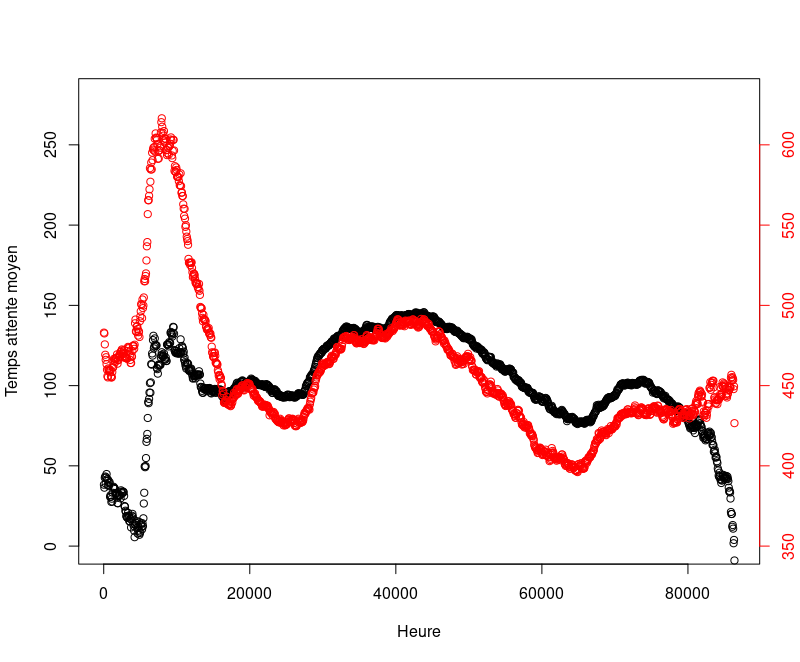
\includegraphics[width=5cm]{TempsAttente}
		\caption{Comparison between waiting time during the taxiing (black) and taxi time (red).}
		\label{waiting}
	\end{subfigure}
	\begin{subfigure}[b]{0.7\textwidth}
		\centering
		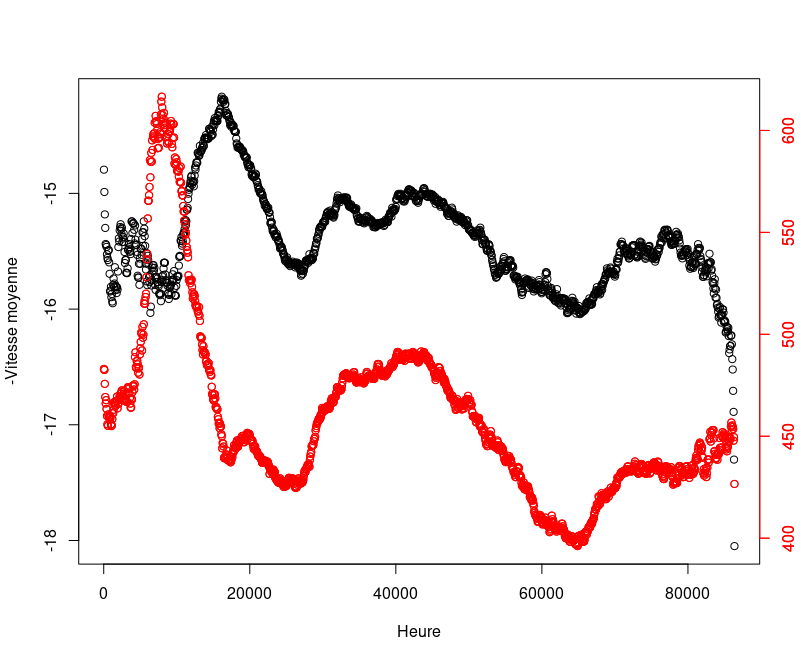
\includegraphics[width=5cm]{Vitesse}
		\caption{Comparison between the opposite (since we expect the taxi time to be inversely proportional to the speed) of average speed during the taxiing (black) and taxi time (red).}
		\label{vitesse}
	\end{subfigure}
	\caption{Behavior of average taxi time as a function of the hour of the day compared to the behavior of parking-runway distance, waiting time and speed.}
	\label{comparisons}
\end{figure}




As we can see from Figure \ref{comparisons}, what explains better the night time peak is the larger distance traveled by the aircraft on average at that hour. Also the waiting time gives a little contribution, while the speed is on average larger in correspondence of the peak. This means that it gives a negative contribution to the taxi time, with respect to the other hours of the day.

From an the interviews with the GC it emerged, in fact, that every night at least a couple of the four runways is closed, alternating the northern and the southern couple every 2 weeks. The runways stay usually closed from midnight to 5 a.m..
Then, the peak of 3 a.m. can be explained if the distance between the stand and the open runway is on average longer than during day time.

This hypothesis is verified in section \ref{comparison}.


\subsection{Comparison between AFR and FDX stands}\label{comparison}

We explored the dependency of taxi time on the runway and on the parking area, with a particular focus on Air France and FedEx flights. 

In fact, the length of the route from the stand to the runway explains not only the fact that the average taxi time for Fed-Ex is longer than the one of Air France, but also the night time peak. In fact, Fed-Ex flights occur usually at night, as shown in table \ref{companiesNight}.



\begin{table}[h!!!!!!!!!!!!!!!!]
	\begin{center}
		\caption{Average company frequencies for the whole day (left) and for the time interval 1:35 a.m. - 3.40 a.m. (right)}
		\label{companiesNight}
		\begin{tabular}{p{1.5cm}p{2cm}} % <-- Alignments: 1st column left, 2nd middle and 3rd right, with vertical lines in between
			\textbf{Company} & \textbf{Frequency whole day}\\
			\hline
			AFR & 48,3\% \\
			EJU & 6,8\% \\
			FDX & 2.25\% \\
		\end{tabular}
		\quad
		\begin{tabular}{p{1.5cm}p{2cm}} % <-- Alignments: 1st column left, 2nd middle and 3rd right, with vertical lines in between
			\textbf{Company} & \textbf{Frequency night time}\\
			\hline
			FDX & 26,8\% \\
			AFR & 26,4\% \\
			ABR & 20,3\% \\
		\end{tabular}
	\end{center}
\end{table}



We expect the taxi time to be larger when the distance between the parking slot and the runway is larger. This is especially evident with FedEx flight, since they all leave from the same parking area, situated at the periphery of the airport platform.

\begin{figure}[h]
	\centering
	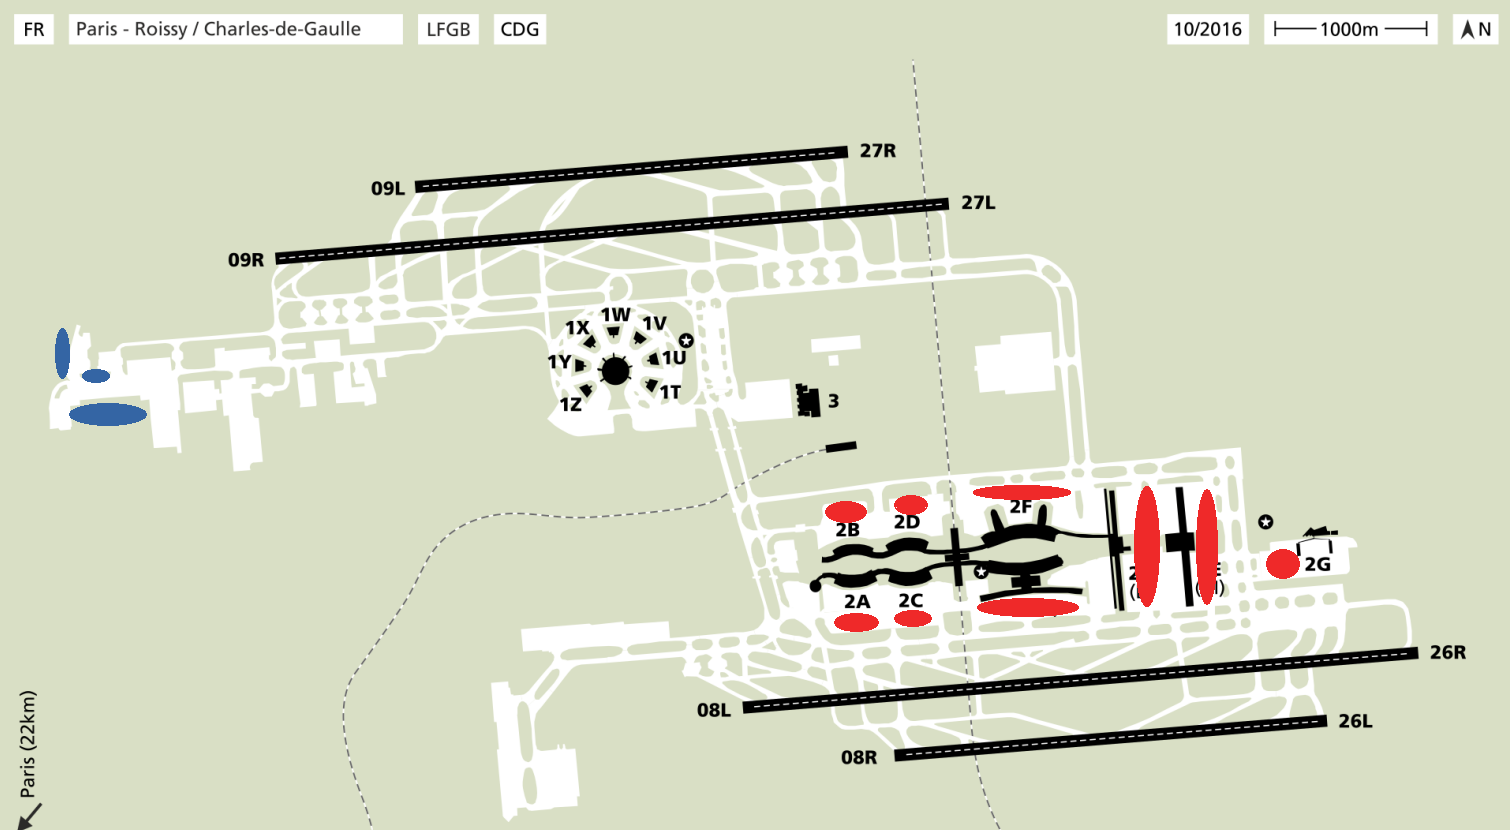
\includegraphics[width=\textwidth]{map_airport_filled}
	\caption{Map of Charles de Gaulle airport. The red ovals correspond to the gates where Air France aircraft usually park. The blue ovals correspond where FedEx aircraft park.}
	\label{map}
\end{figure}

Figure \ref{map} shows a map of the entire airport, where the parking areas for FedEx and AirFrance aircraft are evidenced.
We can see from the map that Air France aircraft have a quicker access to the runways, especially the southern ones ( runways 08L, 08R, 26L, 26R), since their parking position is central. FedEx aircraft, on the other side, have a quite quick access to the northern runways only when they are taking off facing east or landing facing west(runways 09R and 09L). The large distance from the southern runways is the main reason for larger taxi times for FedEx flights.


\subsection{Conclusions and link with ABM}
We showed how the difference in taxi times showed in Figure \ref{companiesFig} can be explained at the first order with the distance between the stands associated with the companies and the runways. The results can explain also the night time peak showed in figure \ref{n_avions}.

The previous results have one main consequence in the implementation of the agent based model: the structure of the airport platform is fundamental to reproduce accurately the real taxi time distribution in our simulation.


\section{Current data analysis: detection of non-standard scenarios}\label{non-standard}
After an interview with the GC, we decided to focus on the detection of non-standard scenarios that occurred in the period of our data set.
In fact, what the GC evidenced was that the main problems occur during high traffic hours and when non-predicted events occur. For the rest of the time, they follow standard procedures described in the ground booklet\cite{livret}.

In standard situation, the rules are followed and the algorithm describing the ground controller decision making process should be quite simple (even if even in standard scenarios they have some decisions to take, such as which entrance/exit to use to/from the runway).
What our current and future data analysis is focused on is the detection of non-standard situations, to be able to isolate them and perform an analysis on the behavior of the GC in these cases.

Below is a list of non-standard scenarios and a possible way to detect them in our data set.
\begin{itemize}
	\item \textbf{Closed taxiway.} They can be detected thanks to the feature ``Cheminement" of our data set, that lists all the main taxiways used by an aircraft during his taxiing procedure, in order. We expect that if a taxiway is closed, it won't be used during a certain time range by any aircraft, even if it is part of the standard path that should have been used.
	\item \textbf{Closed runway.} From an interview to the GC, it emerged that we can distinguish between closure at night time and at day time. At night time, one couple of the four runways is closed, alternating the northern and the southern couple every 2 weeks. At daytime, a runway can be closed for three main reasons: daily inspection(3 times a day, duration 10-20 minutes), inconveniences such as bird strikes (duration 10-30 minutes), technical work that needs to be done at daytime, linked to the radio electric system (duration 1-2 hours).
	
	Runway closure can be detected thanks to the creation of a new variable that represents the time interval between two flights that use the same runway. When this time is too long, the runway can be considered closed.
	\item \textbf{Bad weather conditions.} They can be detected integrating the weather data to our dataset (we asked the dataset to DGAC but they provided only for a dataset of 2 months).
	\item \textbf{De-icing procedures.} There is a variable called ``TempsDegivrage" in our dataset. It is necessary to understand how this variable impacts the eventual delay of flights.
\end{itemize}

Another way of proceeding is to isolate the flight of our data set with a too long taxi time and try to understand what causes it.

\subsection{Detection of runway closure}

We tried to detect the closure of a runway introducing a new variable in our dataset, that indicates the time interval between two consecutive usages of the same runway. To be noticed is the fact that the four runways are indicated with different names, according to the orientation with which they are used. In our analysis we treated as the same runway the couples 26R and 08L (south runway for departures), 26L and 08R (south runway for arrivals), 27R and 09L (north runway for arrivals), 27L and 09R (south runway for departures).

From the table below, we can notice that every day at least one of the four runways were closed for at least one hour, and in the 98\% of the days analyzed at least one runway have been closed for at least four hours, and within those days the majority closures happened from 11 p.m. to 5 a.m..
We see that for 4 times a runway were closed for more than one day. Looking at those data, what emerges is that the southern runway for departures were closed for 4 days from 14/11/19 to 18/11/19, while the southern runway for arrivals were closed for three months, from 07/07/18 to 09/10/18, with an interruption in the closure where a few aircrafts use the runway on 01/08/18 and 05/09/18.

\begin{table}[h!!!!!!!!!!!!!!!]
	\begin{tabular}{C{2cm}|C{2.5cm}|C{2.5cm}|C{2.5cm}}
		\textbf{Time interval (hours)} & \textbf{N of days of closure}& \textbf{N of days of night time closure} & \textbf{N of days of day time closure}\\
		\hline
		1 & 790 (100\%) & 789 (99\%)& 227 (35\%)\\
		2 & 789 (99\%)& 786 (99\%)& 112 (14\%)\\
		3 & 786 (99\%)& 783 (99\%)& 83 (10\%)\\
		4 & 777 (98\%)& 774 (97\%)& 65 (8\%)\\
		5 & 615 (77\%)& 591 (77\%)& 56 (7\%)\\
		6 & 221 (27\%)& 174 (26\%)& 52 (6\%)\\
		7 & 32 (4\%)& 17 (3\%)& 15 (1\%)\\
		24 & 4 (0,5\%)& 2(0,2\%) &2 (0,2\%) \\
	\end{tabular}
	\caption{Table of the occurrences of days in which a closure that lasted more than the time interval indicated in the first column happened. The third column indicates the number of days where the closure occured between 11 p.m. and 5 a.m., the fourth column between 5 a.m. and 11 p.m.. The total number of days analyzed were 790.}
\end{table}


Every flight in the data set is now labeled with the information wether a runway is closed or not. We consider a runway closed if it's not used for more that 30 minutes during daytime (from 6 a.m. to 12 a.m.) or for more than 4 hours during night time (from 12a.m. to 6 a.m.).

\subsubsection*{Further work}
We will have to perform a data analysis that shows the difference in the behavior of aircraft when a runway is closed.

\subsection{Research of the expected runway}

From the interviews with the GCs it emerged that the runway that a flight should use is chosen by the DMAN based on the strategy that the tower supervisor suggests to it. The strategy usually consists in choosing the runway based on the destination (in case of departures) or on the origin (in case of arrivals) to avoid crossings in the sky, since they are a lot more difficult to handle. 

We tried to verify this strategy. We grouped the flights based on their destination or origin, and looked at the percentage of flights that took off or landed from the northern runway and from the southern one, expecting to have extreme values. In fact, if the strategy used for choosing the runway is based on the destination/origin, we expect that almost 100\% of flights with the same destination take off/land on the same runway.

The data showed, on the contrary, that only for 55\% of departing flights to a same destination it is assigned the same runway more than 80\% of the time. For the other destinations, the runway is assigned following criteria that are different from the direction of the destination.

\subsubsection*{Further work}
Interview the tower supervisor or the GCs about the criteria used to choose a runway.

\subsection{Detection of the usage of non-standard taxi paths}

The GC booklet \cite{livret} contains a list of all the standard paths, that link every parking area to every runway. The data set provides for a variable ``Cheminement" that contains the sequence of taxiways used by the aircraft to go from the runway to the parking area and vice versa. Comparing the two, we can detect the cases when the standard path were not used, and use it as a proxy for unexpected events, such as taxiway closure, aircraft stuck on the taxiway, congestion, etc..

Something to be noticed is that the standard paths in the GC booklet contains only the main taxiway to follow, and not the runway entrance and exit to use, which remains at discretion of the ground controller (then, this decision has to be modeled in the ABM).

This analysis has to be completed and the results are not available yet.


\subsection{Inspection of long taxi times}

One of the strategies that could be used to analyze the causes of delays during taxiing is to isolate the flights with a long taxi time and try to detect the causes of it through the data. 

In particular, equation \ref{time-eq} shows that the main contribution to taxi times can be given whether by long distances, low speed or long/high number of waiting times.

These situations can in turn have different causes, that can be operational ones or physical ones. With the data analysis, we aim at detecting operational flaws, and with the ABM at simulating them and finding a solution to them. Physical causes, on the contrary, cannot be solved by the ABM.
Some examples of operational and physical causes of delay are showed in table \ref{causes} .
\begin{table}[h!!!!!!!!!!!!!!!]
	\begin{tabular}{|p{3cm}|p{4cm}|p{4cm}|}
		\hline
		\textbf{Event}& \textbf{Operational causes}& \textbf{Physical causes} \\
		\hline
		Long distances & An aircraft that took the wrong way has to go back, increasing the distance traveled & The stand is far from the runway \\
		\hline
		Low speed & A pilot decides to travel at low speed & Safety constraints in low visibility conditions\\
		\hline
		Long waiting times during taxiing & A potential crossing hasn't been detected soon enough and one aircraft is forced to stop to give way to the other; 
		
		An aircraft is stuck in the taxiway and an alternative path for other aircraft hasn't been elaborated quickly enough & An aircraft gets stuck in the taxiway due to some malfunction \\
		\hline
		Long waiting times at the runway & The runway capacity hasn't been accurately computed, addressing too many aircraft to it & Runway closed\\
		\hline
	\end{tabular}
	\caption{Examples of operational and physical causes of long taxi times.}
	\label{causes}
\end{table}

To detect the main contributor to the long taxi times (and eventually the physical/operational cause), we isolated the flights with taxi times higher than 30 minutes to see, with the intention to analyze the waiting times during taxiing an the one at the runway. But for these flights, the data set showed big inconsistencies. We are still waiting for an answer from the airport crew about this issue.

\subsection{De-icing procedures}
Among our dataset of about one million flights, only 2764 had been de-iced which is not really significant but it occured on 468 days over 790 of our dataset. Then we decided to study the impact of the de-icing on the taxitime. For this purpose, we compared our de-iced flight with a control sample of 2764 non-deiced flights which had been randomly chosen in order to have the same day, year and type of movement (landing or takeoff) distributions. As we can see in figure \ref{fig:TempsRoulage}, the taxitime's distribution is slighty different for our two groups. The mean taxitime is almost five times bigger for the de-iced planes (2119 s) than for the control sample (464 s). 

\begin{figure}[h!]
\captionsetup[subfigure]{justification=centering}
    \begin{subfigure}[t]{.5\textwidth}
        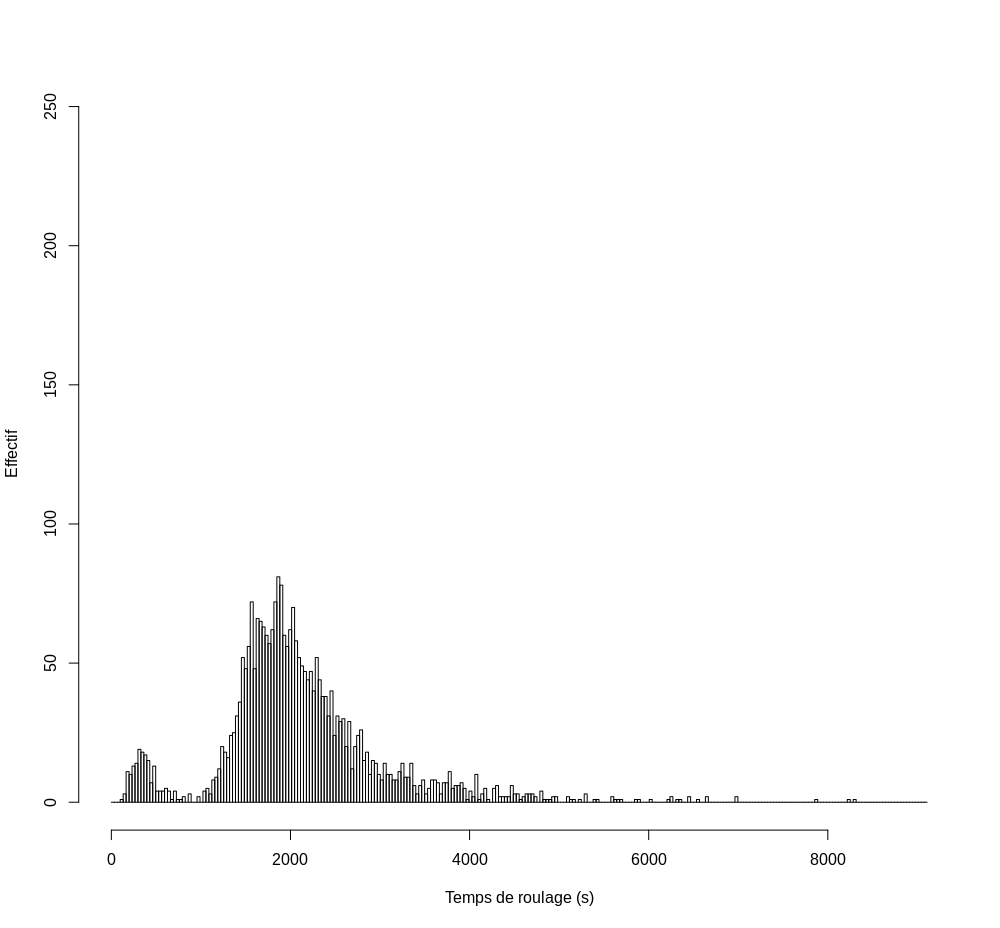
\includegraphics[width = \textwidth]{TempsRoulageDeicing.png}
        \caption{}
        \label{fig:TempsRoulageDeicing}
    \end{subfigure}
    \begin{subfigure}[t]{.5\textwidth}
        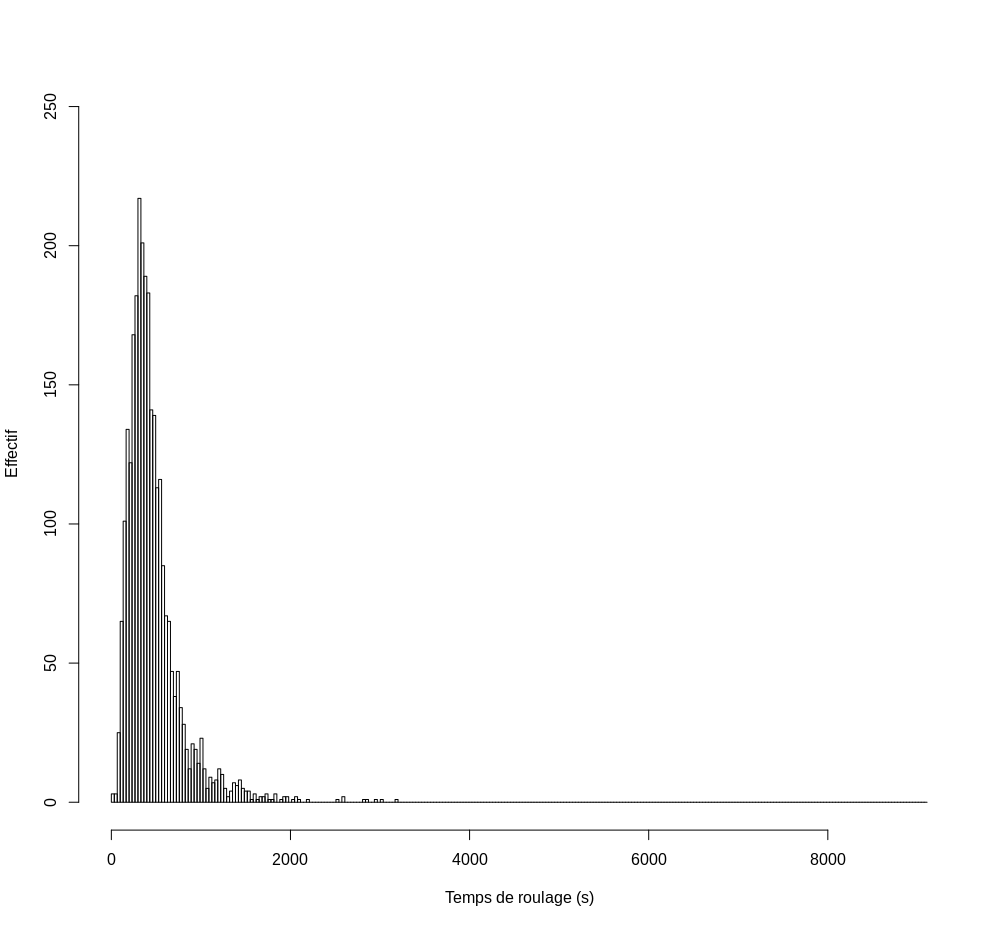
\includegraphics[width = \textwidth]{TempsRoulageControl3.png}
        \caption{}
        \label{fig:TempsRoulageControl3}
    \end{subfigure}
    \caption{Taxitime's distribution for de-iced planes (fig. \ref{fig:TempsRoulageDeicing}) and for the control sample (fig. \ref{fig:TempsRoulageControl3}).}
    \label{fig:TempsRoulage}
\end{figure}

Wa had been informed about the existence of strategies for the de-icing, one of which is to use only one runway in order to concentrate the de-icing procedures on a single place. In order to study this strategy, we identify the uses shows the uses of runways by the de-iced planes and by the planes of the control sample which are shown in table \ref{tab:Deicing}. We will need a deeper analysis of those data to be able to draw a clear conclusion on it. 

\begin{table}[h!]
    \centering
	\begin{tabular}{C{2cm}|C{2.5cm}|C{2.5cm}}
		\textbf{Runway} & \textbf{De-iced planes}& \textbf{Control sample}\\
		\hline
		08L & 23.4\% & 16.9\%\\
		26R & 15.1\% & 30.1\%\\
		08R & 2.0\% & 4.6\%\\
		26L & 4.4\% & 5.1\%\\
		09L & 8.5\% & 4.1\%\\
		27R & 4.5\% & 4.1\%\\
		09R & 22.3\% & 10.8\%\\
		27L & 19.8\% & 23.6\%\\
	\end{tabular}
	\caption{Table of the uses of runways by the de-iced planes and by planes on the control sample.}
	\label{tab:Deicing}
\end{table}
\subsubsection*{Futher work}
We could combine our works on de-icing procedures and standard taxi paths to study if the lengthen of the taxitime is due to the use of a different strategy on the path's and runway's assignations. We also add this topic on our interview's questionnaire. Finally we plan to study bad weather conditions on a broader sens when we would have all of the weather datas.

\newpage
\part{Agent Based Model}

\section{Current agent based model}

The model we developed during the first period of the project is quite simple, and it involves only aircraft agents.

We start with a single runway, 2-terminal airport. Aircrafts arrive at the runway from Terminals 1 and 2, located at distances $d_1$ and $d_2$ from the runway. At each terminal, there is a fixed schedule of departures (eg one plane departs every n time steps). However, this schedule is subject to random variations: each departure time is blurred by some random noise $\eta_i$ (the noise may be depend on Terminal because of gate design / architectural constraints / airlines operating there etc.). On their way from the gate to the runway, aircrafts move at constant speed $v$, so that from Terminal $i$, it takes them a time $t_i = d_i/v$ to get to the runway. However, on their way, they might incur an exponentially distributed delay $\delta_i$. When they arrive at the runway, aircraft enter a queue. With probability $p$, the first aircraft up the queue may have to wait because of inbound traffic (another plane landing). If so, the waiting time is exponentially distributed, with parameter $\lambda$. 
When the first aircraft in the queue takes off, then the next one may either take off immediately afterward, with probability $1-p$, or again, with probability $p$, have to wait because of inbound traffic. 
\smallskip

The model just described is basically a queuing model. When the demand (aircraft arriving at the runway) exceeds the runway capacity, a peak in waiting times at the runway is obtained. This peak partly reproduces the larger waiting time that we have on average during rush hours. 

But given the complexity of the airport platform, this model isn't sufficient. Moreover, it doesn't take advantage of the strength of agent based models, that is the possibility of modeling heterogeneous agents to see if the interaction between them leads to some emergent behaviors of the system.

\section{Ideas for a new ABM}
We would like to build a model in which detailed structural information, namely the airport taxiway structure, are integrated with human/operational factors, namely the strategy followed by the agents involved in the taxiing operations. Both these elements are described in the next sections.

\subsection{Airport structure}

We decided to include a detailed simulation of the airport structure because of the results showed in section \ref{exploratory}. In fact, the mean of the distribution of taxi times depends on the distance traveled by the aircraft, therefore by the position of the stand and of the runway. The airport platform can be modeled as a network whose nodes are the parking areas and the intersection between taxiways, while the edges are the taxi routes. The weight of the edge is going to be equal to the route's length.

To build this kind of network, data about the airport structure are necessary. We required them and we are waiting for an answer from DGAC.

\subsection{Agents and their behaviour}
The objective of the simulation is to reproduce the behavior of the agents involved in the taxiing operations, and eventually find a better strategy. 
The main agents of the simulation are going to be the pilots/aircraft and the ground controllers, but other agents could be included (see section  \ref{other-agents}).

\subsubsection{Ground Controller}

Thanks to an interview with the GC, we are able to describe roughly their behavior and tasks, but further interactions are necessary to examine this topic in depth. 

GC task is leading an aircraft safely from the apron area to the runway entrance. In particular, they take in charge an aircraft at the PAI (point d'arret intermediaire), an area situated at the exit/entrance of the apron area (i.e. the parking area). From the time when the push back starts to the PAI, the aircraft supervised by the apron controller, but the ground controller knows that he is going to manage an aircraft since the beginning of the push back. 

To be noticed is the fact that the time at which an aircraft begins its push back is decided by the DMAN and not by the controllers. This can lead to operational inefficiencies, because the DMAN does not bases its decisions on what is happening on the taxiway. For example, it could happen that an aircraft that just finished its push back cannot travel further because the taxiway is occupied by another aircraft that is doing the push back. Or, as well, a taxiway may be completely blocked because of a stuck aircraft, and instead of waiting for it to be removed at the stand, all the aircraft push back and then queue in the middle of the taxiway. The DMAN showed to increase efficiency \cite{manual}, but there are some improvements that can still be done during unpredictable events.

At the PAI, the exchange between apron and ground controller should be done as quickly as possible, but sometimes delays in this operation can cause waiting time at the PAI. 
The ground controller communicates to the pilots the path they have to follow and the runway they have to use. The last information is suggested by the DMAN based on the strategy that the tower supervisor gives it as an input. The ground controller can decide not to follow the suggestion of DMAN about the runway, but he usually does, especially in high workload situation. 

The ground controller then leads the aircraft to the runway checking if there are conflicts with other aircraft (what does he do if there are conflicts? It's a question for the interview).
Once arrived at the holding point before the runway, the aircraft is taken in charge by the runway controller. In the case landing aircraft, the GC leads the aircraft form the runway to its stand. If the stand isn't free, he has to decide a point on the taxiway where the aircraft can wait.

The interviews with the GC showed that their strategy can be modeled in completely different ways, according to the situation. In particular, identified the following scenarios, associated to the respective behavior:

\begin{itemize}
	\item \textbf{High traffic scenario.} Up to four GC work at the same time in the control tower, each one of them checking over one portion of the airport platform. The GC follow the standard procedures as much as possible. Their strategy is then well defined, and it should usually lead to predictable outcomes. 
	The rules that GC must keep in mind include the following examples \cite{livret}.
	\begin{itemize}
		\item Large aircraft cannot travel along some specific taxiways for safety reasons.
		\item Every parking area has some strict rules that regulate the entrance and the exit of aircraft (one way routes, etc.).
		\item A standard path is associated to every couple \textit{Parking Area, Runway}.
		\item The direction of one way taxiways changes based on the orientation of the runway (face east or west).
	\end{itemize}
	\item \textbf{Low traffic scenario.} This situation happens at night, when one of the two couples of runways is closed. Only one GC is operating, and he controls the whole airport platform. The GC can decide not to follow standard procedures to gain some seconds in taxi times, since there is no danger of accident with other aircraft.
	\item \textbf{Non-standard scenario.} It's the case of bad weather conditions, aircraft stuck in the middle of the taxiway, unexpected runway closure, taxiway closure etc. Expecially in rush hours, the workload for GC in those cases is really high, since they have to think about a solution in a small amount of time. The strategy here is not well defined, and it will be object of further investigation during the interviews.
\end{itemize}

Our model will hopefully include 3 different strategy models for those three different scenarios, that will be investigated thanks to the interviews with the ground controllers.


\subsubsection{Pilots}

Another important agent is the pilot, that will maybe be merged with the agent aircraft to make the model simpler. 

The pilots have the task to inform the controllers when they are ready to push back, to obtain the clearance to begin the push back by the delivery controller.

From the interviews with GC, it emerged that once the taxiing has begun the pilots have little autonomy while taxiing, since they have to follow the path indicated by ground controllers.
Nevertheless, they have the autonomy to choose the speed of taxiing.

\subsection{Further investigation: the interviews}
We have already planned some interviews with GC and pilots. 
They aim at better understand the behavior of both GC and pilot agents. In particular, they will focus on the description of the interactions between pilots and GC, between GC and DMAN and on the degree af autonomy that pilots have with respect to GC and that GC have with respect to DMAN. 

In addition, the interview to the GC will explore their interactions with the tower supervisor and other agents involved in the taxi operations.

\subsection{Doubts: operational range of the simulation and other agents}\label{other-agents}
The complexity of the airport system detailed in section \ref{ACDM} requires a special regard in the choice of the operational range described by the simulation, and of the list of agents involved.

There are many factors that can influence the taxi time. For departures: the schedule of TOBT (decided months before by the aircraft operators and the airport), the TSAT outputted by the DMAN 45 minutes before the push back, the runway chosen by DMAN, the runway capacity that the tower supervisor gives as an input to the DMAN. For arrivals: the time at which the aircraft receives the clearance to land, the availability of stands. For both: the path chosen by GC, the strategy of the GC in response to unexpected events.
Therefore, it is essential to define an operational range that we want to simulate in our ABM, and consequently the list of agents that we want to use. 

In fact, if we decide to improve the TSAT and the parameters given as an input to the DMAN, it is essential to include in our model a DMAN agent, a delivery controller that receives its output and gives the departure clearences, and a tower supervisor agent who set the parameters of the DMAN.

If we chose to focus on the strategy of GC, we will set as parameters the output of DMAN and the tower supervisor decisions about the input parameters of the DMAN. 
In fact, choosing this option we would make the simulation "blind" to what happens to the aircraft before it crosses the PAI and after it arrives at the holding point at the runway, and vice versa. Information about what happens in those time period arrive as a parameter to the GC, and not as an effect of the simulation. 

If we include in the simulation also what happens in the apron area (push-backs that prevent other aircraft to pass, miscommunication between the delivery controller and the pilot, etc.) and at the runway or in the sky (for example, an aircraft that gains precedence because it declares to have run out of fuel), we will need to model the apron controller, the runway controller and the approach controller, with which the GC interact. 

To take this decision, it is essential to understand what are the agents that the GC interact with and what is their role in the taxi time.



\begin{thebibliography}{9}
	
	\bibitem{gotteland}
	J.B. Gotteland,
	\textit{Optimisation du trafic au sol sur les grands aéroports,}
	PhD thesis,Institut National Polytechnique de Toulouse, 
	2004
	
	\bibitem{rathinam}
	S. Rathinam, J. Montoya, and Y. Jung, 
	\textit{An optimization model for reducing aircraft taxi times at the Dallas Fort Worth International Airport,}
	Proceedings of the 26th International Congress of the Aeronautical Sciences, 
	2008
	
	\bibitem{chua}
	Zarrin  K  Chua,  Mickael  Causse,  Mathieu  Cousy, Fabien  André,
	\textit{Modulating   Workload   for   Air   Traffic   Controllers   during   Airport Ground  Operations},
	Human  Factors  and  Ergonomics  Society Annual Meeting,  Oct  2015,  Los  Angeles,  United  States.  59  (1),  pp.16-20 Proceedings  of  the  Human  Factors  and  Ergonomics  Society  Annual Meeting, 
	2015
	
	\bibitem{noortman}
	T. Noortman,
	\textit{Agent-Based Modelling of an Airport’s Ground Surface Movement Operation: Understanding the principles and mechanisms of decentralised control,}
	2018
	
	\bibitem{ACDMimpact}
	EUROCONTROL,
	\textit{A-CDM Impact Assessment}, 
	2016
	
	\bibitem{DMAN}
	DMAN project partners,
	\textit{Basic DMAN Operational Service and Environment Definition (OSED)},
	2011
	
	\bibitem{livret}
	DGAC \& DSNA,
	\textit{Livret Sol CDG},
	2018
	
	\bibitem{manual}
	EUROCONTROL, ACI, IATA,
	\textit{Airport CDM Implementation Manual},
	2017
\end{thebibliography}
	
	
\end{document}